\documentclass[UTF8,a4paper,11pt]{ctexart}

\usepackage{amsmath,amssymb}
\usepackage{booktabs}
\usepackage{graphicx}
\usepackage{geometry}
\usepackage[numbers,sort&compress]{natbib}
\usepackage{hyperref}
\usepackage{fancyhdr}
\usepackage{microtype}
\usepackage{placeins}

\geometry{left=2.45cm,right=2.45cm,top=2.35cm,bottom=2.35cm}
\hypersetup{colorlinks=true,linkcolor=black,citecolor=blue,urlcolor=blue}
\setlength{\parindent}{2em}
\setlength{\parskip}{0.25em}
\linespread{1.22}
\pagestyle{fancy}
\fancyhf{}
\fancyhead[L]{时序知识图谱预测的预序贯答案集校准}
\fancyhead[R]{中文逐字翻译稿}
\fancyfoot[C]{\thepage}
\setlength{\headheight}{14pt}

\newcommand{\cov}{\operatorname{Cov}}

\title{面向时序知识图谱预测的预序贯答案集校准}
\author{王鑫宇\\安徽信息工程学院，安徽芜湖 241000\\\texttt{xywang68@iflytek.com}}
\date{}

\begin{document}
\maketitle

\begin{abstract}
时序知识图谱的预测结果可服务于事件监测及下游决策，但标准排序指标无法说明返回的答案集是否能以给定概率覆盖数据中记录的真实答案。现有面向知识图谱的共形方法主要校准静态链接预测。那么，校准过程能否只使用此前已经揭示的时间戳批次，在保持时间顺序的条件下修复可靠性；这种修复又需要付出怎样的效用代价？本文采用一种控制信息泄漏的预测序贯协议研究这一问题，而不声称在任意漂移下仍具有有效性。评估覆盖 ICEWS14 和 ICEWS05-15、两个采用统一协议的评分器系列、五个随机种子、四种分数变换、三种历史策略、受控训练事实删除以及过滤负采样敏感性。在删除 30\% 训练事实且目标覆盖率为 0.90 时，滚动边际校准的观测标签覆盖率为 0.8988--0.9002。相对于固定的静态边际阈值，其覆盖率提高 0.0798--0.1025，但每个预测集增加 1158--2038 个实体。因子消融表明，历史策略与分数几何存在交互：相对滚动边际，滚动 Minmax 可减少 1091--1773 个实体，但覆盖率影响随数据集而变；滚动 Softmax 则出现过度覆盖，并增加 2081--4991 个实体。训练事实删除和所检验的负采样方案都无法解释主要的可靠性差距。多答案查询的全集覆盖率仍明显低于单答案查询，而查询最大值校准目标还会使全集覆盖率进一步下降 0.0011--0.0081。因此，近期历史校准可作为有用的时序可靠性诊断工具，但并非始终高效，也不具备普遍有效性。
\end{abstract}

\noindent\textbf{关键词：}时序知识图谱；链接预测；共形预测；预测序贯评估；不确定性量化；答案集；时序漂移

\section{引言}

时序知识图谱（temporal knowledge graph，TKG）用带时间戳的关系表示实体之间的联系。它们可以支持对未来交互和事件的预测，尤其适用于这样一类场景：漏掉一个可能答案的代价可能高于检查一个候选短名单的代价。然而，大多数 TKG 模型仍使用过滤平均倒数排名（MRR）和 Hits@\(K\) 进行评价\cite{garciaduran2018sequence,li2021regcn,li2022tirgn,cai2023survey}。这些指标评价的是排序，却不能回答另一个操作层面的问题：一个标称覆盖率为 \(1-\alpha\) 的返回集合，是否确实能以该比例包含数据中记录的正确实体？

共形预测可以把模型分数转换为预测集，并且不要求建立参数化的标签概率模型\cite{vovk2005algorithmic,angelopoulos2023gentle}。KGCP 将拆分共形预测用于静态知识图谱嵌入，CondKGCP 则研究谓词条件下的答案集\cite{zhu2025kgcp,zhu2025condkgcp}。时序预测改变了信息结构：校准发生在测试流之前，分数分布可能随时间演化，而且在时间戳 \(t\) 观测到的标签不能影响同一时间戳内的另一项预测。因此，即使排序模型本身保持不变，一个固定阈值也可能不再可靠。

本文提出的问题是：\emph{只根据严格早于当前时间戳的批次更新答案集阈值，能否修复时序可靠性；这种修复在集合大小和子群表现上需要付出什么代价？}为回答这一问题，本文采用按时间戳分批的预测序贯协议。冻结的评分器首先输出时间 \(t\) 的全部主语侧和宾语侧预测，然后才把该批次的标签释放给校准历史。本文将静态历史、扩展历史和近期滚动历史与四种不合规分数交叉组合，从而避免将历史策略的影响与分数几何的影响混为一谈。

本文证据比单模型案例研究更广，但仍有意维持受控范围。主实验矩阵覆盖 ICEWS14 和 ICEWS05-15、时序 DistMult 和一个采用统一协议的连续时间复数评分器、五个随机种子，以及最高 30\% 的训练事实删除。配对敏感性实验比较过滤训练负样本与均匀训练负样本。后续因子分析复用经过核验的检查点，在三种历史策略下评估四种分数。主矩阵共包含 90 个已完成的随机种子--删除率条件；因子分析包含 20 个数据集--评分器--随机种子案例，以及 131,550 行时间戳--方法结果。

本文有三项主要发现。第一，在全部四个数据集--评分器案例中，近期历史边际阈值均能修复固定边际阈值的严重覆盖不足，但需要显著更大的预测集。第二，最优的可靠性--效用权衡并不随分数函数或数据集保持稳定：Minmax 在 ICEWS14 上明显更小，而 Softmax 在滚动更新下变得低效且过度保守。第三，标签层面的边际覆盖率掩盖了显著的多答案缺口，最直接的查询最大值校准尝试也未能修复这一问题。本文的贡献在于一个控制信息泄漏的诊断协议、一份对其失效模式进行因子分解的实证分析，以及对现有证据能够支持何种时序共形结论的明确界定。本文不提出针对任意时序漂移的新分布无关定理。

\section{相关工作}

\textbf{时序知识图谱预测。}
TKG 补全方法包括时序序列编码器、张量分解以及循环图网络\cite{garciaduran2018sequence,lacroix2020tcomplex,li2021regcn,li2022tirgn}。简单的历史基线仍可能具有竞争力，这使得数据划分设计和时序信息控制成为评估的核心\cite{gastinger2024repeat,gastinger2024tgb2}。本文的校准层接收冻结的全实体分数向量，并不改变候选排序。因此，下文使用的两个评分器系列是受控协议下的变体，而不是新的预测架构。

\textbf{图输出的共形预测。}
概率校准已在神经分类器和知识图谱嵌入中得到研究\cite{guo2017calibration,safavi2020calibration}。KGCP 使用 NegScore、查询级 Minmax 和 Softmax 变换为链接预测构造答案集\cite{zhu2025kgcp}；CondKGCP 则从边际行为进一步转向谓词条件行为\cite{zhu2025condkgcp}。APS 和 RAPS 在多分类预测中利用按排名累积的概率质量权衡覆盖率和集合大小\cite{angelopoulos2021raps}。这些研究说明，分数设计是首要实验因素，而非无关紧要的实现选择。

CFEP 最近通过分数扩散和学习得到的分位数权重，研究了时序知识图谱上的共形事件类型预测\cite{hu2026cfep}。本文的估计目标和协议均与其不同：本文研究链接预测中的实体答案集，冻结评分器，并分离仅使用过去信息的历史策略与分数几何对校准的影响。本文目标是诊断性的，即报告简单时序更新在何处有效、代价是什么，以及在何处失效。

\textbf{非交换条件下的校准。}
加权共形预测、自适应共形推断，以及针对非交换数据的分析，能够在特定漂移或在线反馈条件下给出保证\cite{tibshirani2019covariate,gibbs2021adaptive,barber2023beyond,farinhas2024nexcrc}。NCPNET 研究非交换的时序图神经网络\cite{wang2025ncpnet}。本文的滚动规则有意保持简单：它根据最近已揭示的分数估计经验分位数。由于它既不使用似然比权重，也不假设有界漂移过程，因此不能把交换条件下的覆盖率保证直接移植到测试流。

\section{问题、校准与保证边界}

\subsection{时序查询与可靠性目标}

设 \(\mathcal{E}\) 和 \(\mathcal{R}\) 分别为封闭的实体词表和关系词表。一个 TKG 由四元组 \((s,r,o,t)\) 构成。本文将宾语查询写为 \(x=(s,r,\square,t)\)，其中 \(\square\) 表示待预测的实体位置；主语预测则表示为 \((o,r^{-1},\square,t)\)。对于查询 \(x\)，令 \(A_t(x)\subseteq\mathcal{E}\) 表示时间戳 \(t\) 上所有记录到的答案，令 \(C_t(x)\) 表示预测答案集。

首要可靠性估计量是观测标签覆盖率：
\[
  \widehat{\cov}_{\mathrm{label}}
  =\frac{1}{N}\sum_{(x,y)}\mathbb{1}\{y\in C_t(x)\}.
\]
它不同于全集查询覆盖事件 \(\mathbb{1}\{A_t(x)\subseteq C_t(x)\}\)。本文同时报告二者，并报告平均集合大小、过滤 MRR，以及部分答案召回率 \(|A_t(x)\cap C_t(x)|/|A_t(x)|\)。每个指标都只涉及基准数据中记录的标签，而不代表数据之外所有可能为真的事件。

\subsection{分数与历史策略}

令 \(f_\theta(x,y)\) 为冻结 TKG 模型给实体 \(y\) 分配的分数。边际不合规分数为
\[
 a_{\mathrm{margin}}(x,y)=\max_{z\in\mathcal{E}}f_\theta(x,z)-f_\theta(x,y),
 \qquad C_q(x)=\{y:a(x,y)\le q\}.
 \tag{1}\label{zh:eq:margin}
\]
对于校准分数 \(a_1,\ldots,a_n\) 和目标覆盖率 \(1-\alpha\)，令
\[
 k=\min\{n,\lceil(n+1)(1-\alpha)\rceil\},\qquad q=a_{(k)}.
 \tag{2}\label{zh:eq:quantile}
\]
静态历史只根据初始校准阶段的最后一个区间估计一次 \(q\)。扩展历史使用当前时间戳之前已经揭示的全部分数。滚动历史使用最近 \(W=1000\) 个已经揭示的分数。

为了区分分数与历史，因子研究还评估 KGCP 使用的三种变换。对于分数向量 \(f\)，
\[
\begin{aligned}
 a_{\mathrm{Neg}}(y)&=-f_y,\\
 a_{\mathrm{Minmax}}(y)&=-\frac{f_y-\min_z f_z}{\max_z f_z-\min_z f_z},\\
 a_{\mathrm{Softmax}}(y)&=1-\frac{\exp(f_y/T)}{\sum_z\exp(f_z/T)},
\end{aligned}
\tag{3}\label{zh:eq:scores}
\]
其中，取值范围为零的 Minmax 向量映射为零，且 \(T=1\)。本文在统一的数据划分和评分器下复现这些已发表的分数定义，但不声称复现 KGCP 的完整训练流程。

在时间戳 \(t\)，所有查询分数、阈值和预测集都在该时间戳的任何标签被释放之前保存。随后，整个批次才被加入扩展历史和滚动历史。这一顺序可防止同一时间戳内的信息泄漏。

\subsection{覆盖率边界与集合几何}

第一个定理给出熟知的交换性参考基准，时序实验应据此解读。列出这一结果的目的，是明确在按时间顺序划分后，通常共形论证中的哪一部分不再成立\cite{vovk2005algorithmic,angelopoulos2023gentle}。

\noindent\textbf{定理 1（交换条件下的拆分共形参考结果）。}\quad
在冻结评分器的条件下，假设 \(a_1,\ldots,a_n,a_{n+1}\) 可交换，且 \(\alpha\ge 1/(n+1)\)。采用式~\eqref{zh:eq:quantile} 中的 \(q\)，有
\[
 \Pr\{a_{n+1}\le q\}\ge 1-\alpha.
 \tag{4}\label{zh:eq:exchangeable}
\]
如果这些分数几乎必然互不相同，则覆盖率至多为 \(1-\alpha+1/(n+1)\)。

\emph{证明。}
交换性使 \(a_{n+1}\) 在这 \(n+1\) 个分数中的排名服从均匀分布。该排名不超过 \(\lceil(n+1)(1-\alpha)\rceil\) 的事件，其概率至少为 \(1-\alpha\)。使用校准顺序统计量只可能进一步纳入与测试分数相同的并列值；不存在并列时，下一个可达到的排名最多贡献 \(1/(n+1)\)。\hfill\(\square\)

时序顺序不一定满足定理 1 的前提。下一个结果并不会恢复该保证，而是分解经验阈值的误差。在给定时间 \(t\) 之前全部可用信息的条件下，令 \(F_t\) 为当前观测标签分数的累积分布函数，令 \(\widehat H_t\) 为选定历史分数池的经验累积分布函数，令 \(H_t\) 为该分数池的参考累积分布函数。定义
\[
 \delta_t=\sup_u|F_t(u)-H_t(u)|,\qquad
 \epsilon_t=\sup_u|\widehat H_t(u)-H_t(u)|.
\]
令 \(\eta_t=\widehat H_t(q_t)-\widehat H_t(q_t^-)\) 表示所选阈值处的经验并列质量，并令 \(\rho_{n,\alpha}=\max\{0,(k-1)/n-(1-\alpha)\}\)。

\noindent\textbf{定理 2（确定性的时序失配分解）。}\quad
对于式~\eqref{zh:eq:quantile} 中的闭区间阈值，有
\[
 1-\alpha-\delta_t-\epsilon_t
 \le F_t(q_t)\le
 1-\alpha+\rho_{n,\alpha}+\eta_t+\delta_t+\epsilon_t,
 \tag{5}\label{zh:eq:decomposition}
\]
其中上下界均截断到 \([0,1]\) 内。

\emph{证明。}
根据构造，\(\widehat H_t(q_t)\ge k/n\ge1-\alpha\)。两次应用上确界范数界即可得到下界。在 \(q_t\) 之前，严格小于它的经验观测至多有 \(k-1\) 个，因此 \(\widehat H_t(q_t)\le(k-1)/n+\eta_t\)。再次应用同样的两个偏差界即可得到上界。\hfill\(\square\)

该分解揭示了一种权衡。更短的历史可能减小时间失配 \(\delta_t\)，却可能增大经验误差 \(\epsilon_t\) 或离散原子 \(\eta_t\) 的影响。本文并不把这些项估计为新的保证，而是通过覆盖率和集合大小衡量它们的可观测后果。

\noindent\textbf{命题 1（集合嵌套与多答案判据）。}\quad
对于任意不合规分数，若 \(q_1\le q_2\)，则 \(C_{q_1}(x)\subseteq C_{q_2}(x)\)。对于边际不合规分数及 \(q\ge0\)，预测集非空。此外，
\[
 A_t(x)\subseteq C_q(x)
 \quad\Longleftrightarrow\quad
 \max_{y\in A_t(x)}a(x,y)\le q.
 \tag{6}\label{zh:eq:querymax}
\]

\emph{证明。}
预测集是不合规分数的次水平集，因此具有嵌套性。根据式~\eqref{zh:eq:margin}，得分最高的实体具有零不合规分数。最后一个等价关系成立，是因为当且仅当所有已记录答案中最大的不合规分数不超过阈值时，每个已记录答案都会被纳入。\hfill\(\square\)

式~\eqref{zh:eq:querymax} 启发了查询最大值校准目标，但它并不意味着相应经验阈值一定优于标签层面的阈值：从标签切换到唯一查询，会同时改变样本量和顺序统计量。本文直接检验这一区别。

\section{实验与结果}

\subsection{研究设计}

实验回答四个问题。\textbf{RQ1} 考察近期历史校准能否跨数据集和评分器修复静态覆盖不足。\textbf{RQ2} 将历史策略与分数几何分离，并测量相应的效用代价。\textbf{RQ3} 检验训练事实删除或过滤负采样能否解释主要效应。\textbf{RQ4} 测量多答案可靠性，并检验命题 1 引出的查询最大值目标。

ICEWS14 和 ICEWS05-15 是由 ICEWS 编码事件数据构建的事件图\cite{boschee2015icews}。表~\ref{zh:tab:data} 给出规范化后的图规模。本文对唯一时间戳进行排序：最早的 60\% 用于训练评分器，随后 20\% 提供互不重叠的验证与校准用途，最后 20\% 构成测试流。中间区间继续按时间顺序划分为：25\% 用于评分器验证，30\% 用于校准器调优，15\% 用于选择器验证，30\% 用于最终初始校准。

\begin{table}[htbp]
\centering
\caption{规范化后的数据集统计。关系数不包括内部用于主语预测的逆关系副本。}
\label{zh:tab:data}
\begin{tabular}{lrrrr}
\toprule
数据集 & 实体数 & 关系数 & 事实数 & 时间戳数\\
\midrule
ICEWS14 & 7,128 & 230 & 90,730 & 365\\
ICEWS05-15 & 10,488 & 251 & 461,329 & 4,017\\
\bottomrule
\end{tabular}
\end{table}

时序 DistMult 使用 256 维实数嵌入。第二个评分器使用 128 维复数嵌入，以及由常数、线性、二次、正弦和余弦特征组成的共享连续时间映射。它是采用统一协议的 ComplEx 风格替代评分器，而不是官方 TComplEx 或 TNTComplEx 优化器。两个评分器都使用相同的成对 softplus 目标函数、Adam 优化器、\(10^{-3}\) 学习率、\(10^{-6}\) 权重衰减、1024 的批大小、128 个负样本、最多 200 个训练轮次，以及基于验证集的早停。

主实验矩阵使用过滤训练负样本，随机种子为 17、29、43、59 和 71。ICEWS14 在删除率 0、0.1、0.2 和 0.3 下使用两个评分器。ICEWS05-15 的 DistMult 使用全部四个删除率，连续时间复数评分器使用删除率 0 和 0.3。删除只作用于训练事实；如果均匀删除会移除某个实体在训练集中的全部出现，则保留该实体最早的一次出现。配对的均匀负采样敏感性实验分别在 ICEWS05-15 DistMult 和 ICEWS14 连续时间复数评分器上进行，删除率为 0 和 0.3。过滤负样本会排除训练图中保留的正例，而且不会查询未来事实。

后续因子实验固定删除率为 0.3，使用过滤负样本，并为四个数据集--评分器案例中的每个案例和五个随机种子复用经过核验的检查点。它将式~\eqref{zh:eq:scores} 中的四种分数与静态、扩展和滚动三种历史交叉组合，还在同样三种历史下评估查询最大值边际。任何测试结果都不用于选择分数或历史策略。

目标覆盖率为 0.90。主要区间采用 20,000 次等随机种子加权的循环移动块自助法重复，块长为七个时间戳；块长 3、14 和 21 用于检验结论对依赖尺度的敏感性。对比按随机种子和时间戳配对。代码、解析后的配置、派生结果表、图表脚本和校验和可在 \url{https://github.com/xywang815/riskcal-tkg-w} 获取。ICEWS 原始数据可从 \url{https://doi.org/10.7910/DVN/28075} 以及仓库中记录的公开基准来源获取。

\subsection{RQ1：近期历史修复静态边际覆盖不足}

图~\ref{zh:fig:generalization} 首先展示跨数据集规律。在删除 30\% 训练事实时，ICEWS14 上 DistMult 和连续时间复数评分器的滚动边际覆盖率分别为 0.8996 和 0.8988；ICEWS05-15 上两个评分器的该指标均为 0.9002。相应的滚动减静态配对增益依次为 0.0798（95\% CI [0.0621, 0.1006]）、0.0802（[0.0612, 0.1014]）、0.1011（[0.0921, 0.1102]）和 0.1025（[0.0938, 0.1111]）。对应的过滤 MRR 分别为 0.3103、0.3129、0.3269 和 0.3295；校准改变答案集成员，但不会改变这一排序。

\begin{figure}[htbp]
\centering
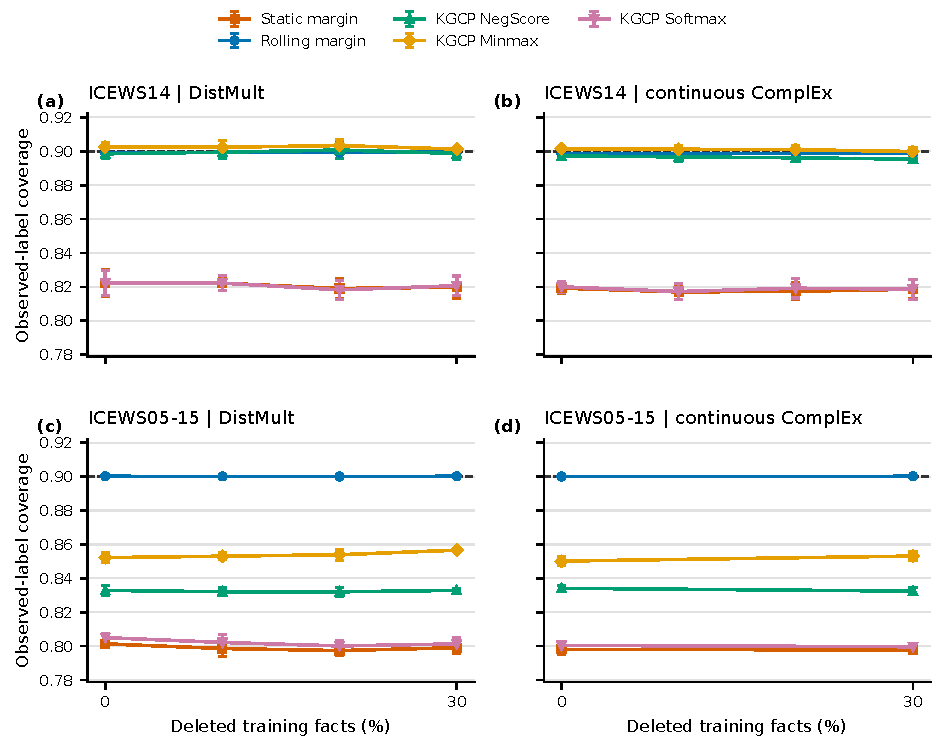
\includegraphics[width=\textwidth]{figures/expansion/expansion_generalization.pdf}
\caption{不同删除率下的观测标签覆盖率。点表示五个随机种子的均值，误差线表示一个随机种子标准差，虚线为 0.90 的目标。ICEWS05-15 连续时间复数评分器只在删除率 0 和 0.3 下评估。每个子图内的方法共享同一个评分器。}
\label{zh:fig:generalization}
\end{figure}

这种修复并非没有代价。在因子化后续实验中，相对静态边际，滚动边际使 ICEWS14 DistMult 的平均集合大小增加 1175 个实体（95\% CI [959, 1416]），使 ICEWS14 连续时间复数评分器增加 1158 个实体（[947, 1382]），使 ICEWS05-15 DistMult 增加 2026 个实体（[1867, 2183]），使 ICEWS05-15 连续时间复数评分器增加 2038 个实体（[1888, 2182]）。在每个案例和每个检验过的块长下，绝对目标误差的减少均为正，集合大小的增加也均为正。因此，可靠的结论是：结果朝目标方向移动，同时伴随显著的效率损失。

\subsection{RQ2：历史策略与分数几何存在交互}

图~\ref{zh:fig:factorial} 将初始研究中耦合的两个组成因素分开。历史从静态变为扩展再变为滚动时，边际分数和 Softmax 明显变化。在 ICEWS14 上，NegScore 和 Minmax 相对稳定，因为它们的静态阈值已接近 0.90。在 ICEWS05-15 上，四种分数都对历史选择作出响应，但分布在覆盖率--集合大小平面的不同区域。

\begin{figure}[htbp]
\centering
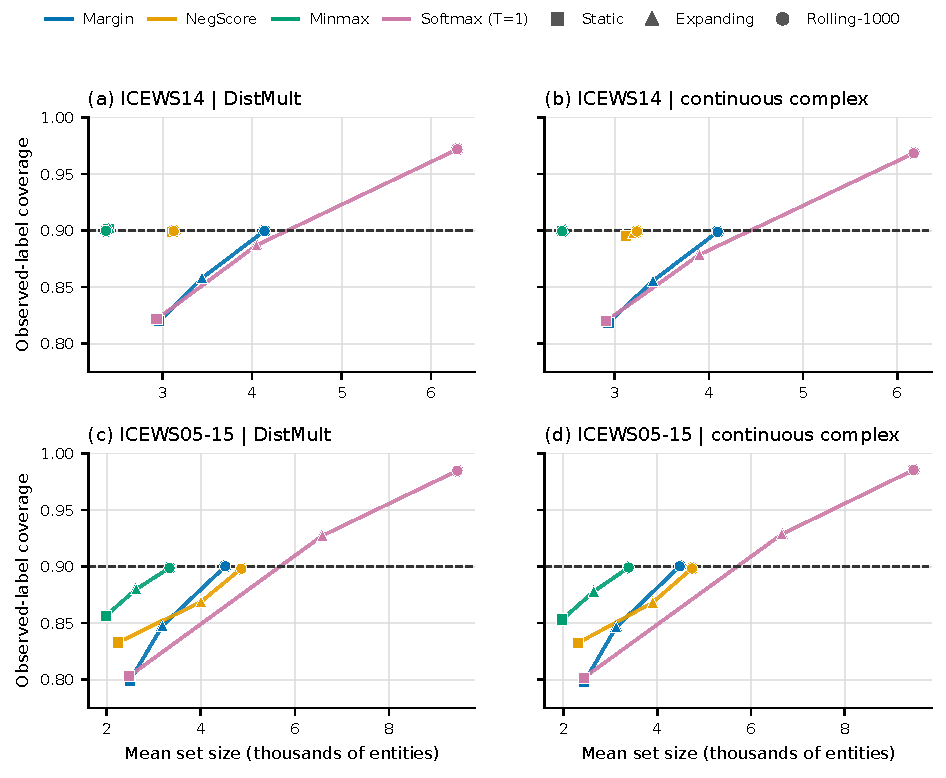
\includegraphics[width=\textwidth]{figures/followup/followup_factorial.pdf}
\caption{删除率为 30\% 时，不合规分数和校准历史的因子消融。每条彩色路径连接一种分数在静态历史（方形）、扩展历史（三角形）和滚动 1000 历史（圆形）下的结果。虚线为 0.90 的目标。数值为等随机种子加权均值；配对不确定性在正文中报告。}
\label{zh:fig:factorial}
\end{figure}

在滚动历史内部，相对边际分数，Minmax 在两个 ICEWS14 案例中的覆盖率仅变化 0.0001 和 0.0005，两个 95\% 区间都跨越零，而平均集合大小分别减少 1773 和 1650 个实体。在 ICEWS05-15 上，集合大小分别减少 1187 和 1091 个实体，但覆盖率变化为 -0.0014 和 -0.0011；这些微小变化对块长敏感。NegScore 呈现同样的数据集依赖：在 ICEWS14 上集合更小，覆盖率变化未能得到确定结论；在 ICEWS05-15 上可靠性略低，而且集合并非始终更小。

Softmax 说明了为什么仅看覆盖率并不充分。在滚动历史下，它相对边际分数把覆盖率提高 0.069--0.085，却增加 2081--4991 个实体。由此得到的覆盖率为 0.9683--0.9854，表现为过度保守，并且在较大图上几乎失去筛选价值。没有一种分数函数在所有案例中占优；必须联合评估分数几何与时序历史。

另一个 ICEWS14 DistMult 短名单诊断通过不同构造得出了相同的谨慎结论。一个通过验证集选择的 RAPS 风格滚动规则使用 Softmax 温度 \(T=1\)、选择容差 0.02，以及固定的 21 个候选网格。该网格由 APS 加上 \(k\in\{50,100,250,500,1000\}\) 与 \(\lambda\in\{10^{-4},5\times10^{-4},10^{-3},2\times10^{-3}\}\) 的组合构成。全部 20 个随机种子--删除率条件都选择了 \(k=50\) 和 \(\lambda=10^{-4}\)。在删除率为 30\% 时，它把平均集合大小从滚动边际的 4069.4 降至 3319.0，同时把观测标签覆盖率从 0.8998 改变为 0.8987；全集查询覆盖率则从 0.9020 降至 0.8874。这只是单一评分器下的效率诊断，不能作为普遍改进的证据。

\subsection{RQ3：所检验的数据干预无法解释该差距}

图~\ref{zh:fig:diagnostics} 将历史效应与两个候选机制区分开。对于 30\% 减去 0\% 的删除效应，每个静态边际和滚动边际覆盖率区间都跨越零。静态变化范围为 -0.0024 至 -0.0004，滚动变化范围为 0.0000 至 0.0005。因此，训练事实删除可以作为评分器压力测试，但实验并不支持它是静态校准失效的原因。

在四个配对条件中，过滤减均匀采样对滚动校准的影响也都跨越零。只有 ICEWS05-15 DistMult 在无删除时出现了较小的正静态边际效应（0.0020 [0.0005, 0.0038]）；其余静态区间均无法得出确定结论。主要历史效应不能归因于本文检验的负采样方案。

\begin{figure}[htbp]
\centering
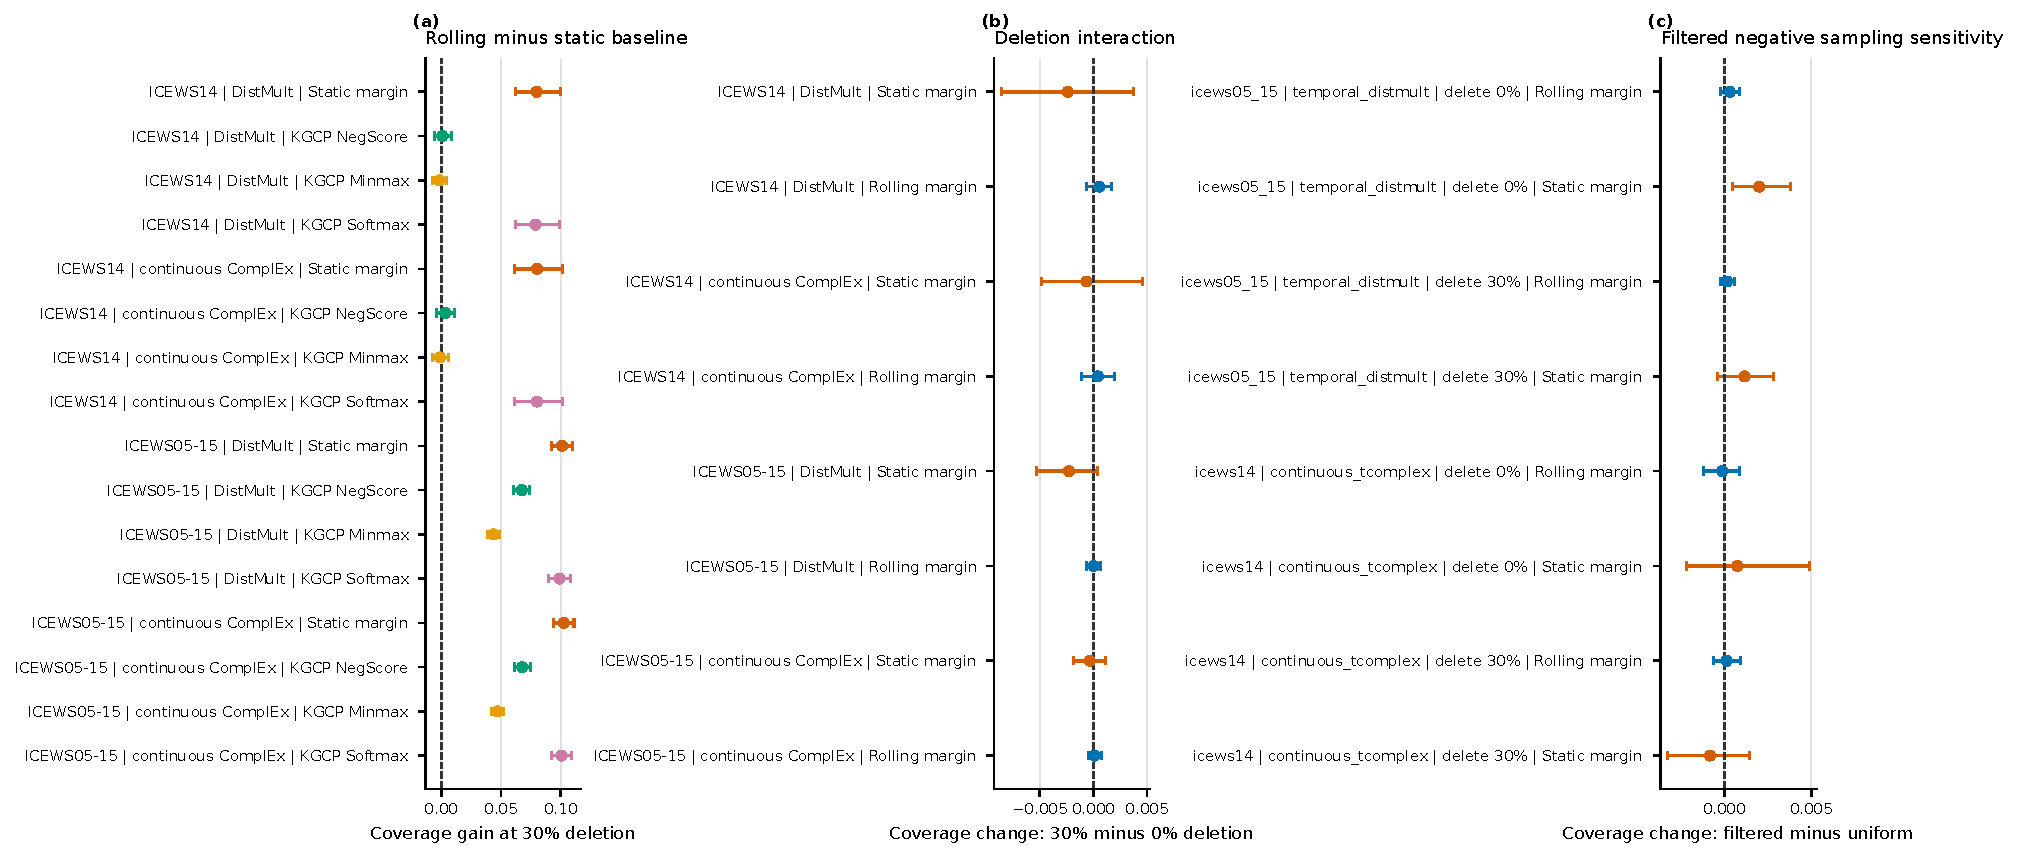
\includegraphics[width=0.97\textwidth]{figures/expansion/expansion_reviewer_diagnostics.pdf}
\caption{配对时间戳块自助法诊断（20,000 次重复；七时间戳块）。（\textbf{a}）删除率为 30\% 时，滚动方法相对静态基线的覆盖率。（\textbf{b}）删除 30\% 而非 0\% 训练事实所导致的覆盖率变化。（\textbf{c}）采用过滤而非均匀训练负样本所导致的覆盖率变化。跨越零的区间不能得出确定结论。}
\label{zh:fig:diagnostics}
\end{figure}

\subsection{RQ4：标签覆盖率掩盖多答案失效}

在因子化后续实验中，采用滚动标签边际校准时，每个案例的多答案全集覆盖率都低于单答案覆盖率：对于 DistMult 和连续时间复数评分器，ICEWS14 上的平均差距分别为 -0.2773 和 -0.3015，ICEWS05-15 上分别为 -0.2059 和 -0.2137。因此，接近 0.90 的标签边际覆盖率并不意味着预测集包含一个查询的全部已记录答案。

命题 1 提示可以对每个已记录答案集的最大不合规分数进行校准。实证结果表明，这一直接查询最大值规则并没有解决问题（图~\ref{zh:fig:queryobjective}）。相对标签层面的滚动边际，其在 ICEWS14 上使全集覆盖率分别变化 -0.0081（95\% CI [-0.0107, -0.0058]）和 -0.0070（[-0.0093, -0.0049]）。ICEWS05-15 上的变化分别为 -0.0011（[-0.0022, 0.0001]）和 -0.0014（[-0.0024, -0.0003]）。预测集减少 39--141 个实体，但多答案差距变得更负。从标签变为唯一查询会减少校准单元数量，并改变经验分位数；这一变化足以抵消最大值分数表面上的保守性。

\begin{figure}[htbp]
\centering
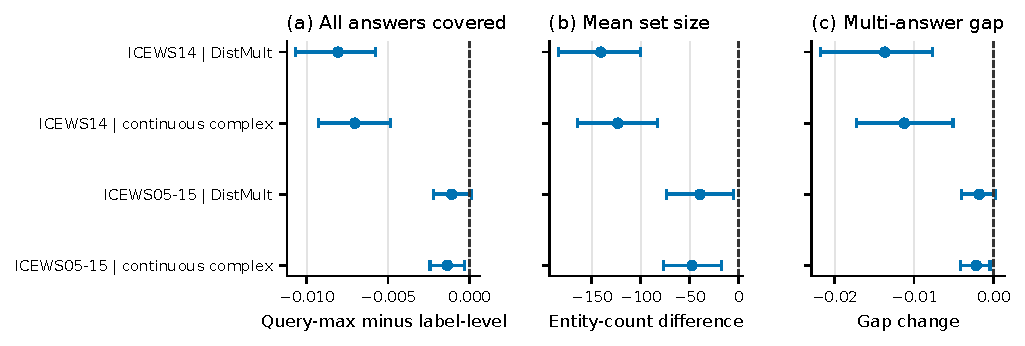
\includegraphics[width=\textwidth]{figures/followup/followup_query_objective.pdf}
\caption{删除率为 30\% 时，查询最大值滚动边际减去标签层面滚动边际的结果。点表示配对效应，误差线表示 95\% 循环移动块自助区间。三个子图分别报告全集查询覆盖率、平均集合大小以及多答案减单答案的覆盖率差距。子图（\textbf{a}）和（\textbf{c}）中的负值表示更差的查询级可靠性。}
\label{zh:fig:queryobjective}
\end{figure}

\section{讨论与结论}

核心结果比普遍方法声明更窄，也更有实际解释价值。当边际阈值在早期固定时，按时间顺序到达的后续测试流覆盖率下降到约 0.80--0.82。使用最近且严格属于过去的分数重新估计阈值后，两个 ICEWS 数据集和两个受控评分器系列上的总体观测标签覆盖率都恢复到接近 0.90。定理 2 提供了相应的诊断性解释：近期历史可能缩小历史分数参考分布与当前分数分布之间的差异。数据并未直接识别这一差异项，因此也不能推出任意漂移下的覆盖率保证。

因子消融改变了这一结果的使用方式。对边际分数而言，滚动更新起决定性作用；但分数变换的影响可能与历史同样大。Minmax 在 ICEWS14 上高效得多，而它在 ICEWS05-15 上的覆盖率影响则较为混合。滚动 Softmax 通过返回实体词表中的大部分实体获得更高覆盖率。因而，部署规则应从可靠性--效用的联合前沿中选择，而不能只根据覆盖率或平均集合大小选择。

两个负结果进一步限制了对机制的解释。删除最多 30\% 的训练事实没有可测量地恶化静态覆盖率；在配对敏感性实验中，过滤训练负样本的影响也很小。因此，为更新阈值提供依据的是时序失配，而不是本文所检验的图损坏。多答案分析还暴露了另一个估计目标失效：标签边际校准可能表现尚可，但“所有答案均被包含”这一事件仍不可靠。简单的查询最大值分数不足以解决问题，因为其校准样本量和分位数会同时改变。

本研究主要有四项边界。ICEWS14 和 ICEWS05-15 都是政治事件图，因此不能建立跨领域的普遍性。第二个评分器是采用统一协议的连续时间复数模型，而不是官方 TComplEx 或 TNTComplEx 的复现。必须作出这一区分，因为已发表 TKBC 预处理使训练、验证和测试共享同一组离散时间支持，而本文协议要求未见过的未来时间戳；为每个未来时间配备自由嵌入的模型，在这些时间上要么没有经过训练，要么会泄漏时序信息。同样，KGCP 对比复用了已发表的分数变换，而不是作者的完整训练流程。最后，五个随机种子限制了对优化随机性的推断，移动块自助法也只能近似数据的依赖结构。

这些边界指向了具体的下一步检验。时序答案集校准应在非 ICEWS 领域上，结合具备归纳或外推能力的 TKG 骨干模型进行评估。结构化校准目标应保持查询层面的样本量，或显式建模答案多重性。谓词条件时序规则可能减轻边际覆盖率所掩盖的大幅关系和方向异质性。对于大型实体词表，任何可靠性提升都必须与候选生成或检索方法结合，以限制全实体评分的代价。

总而言之，近期历史预测序贯校准修复了一个可复现的总体覆盖不足模式，但代价是每个预测集增加数千个候选实体，并且多答案可靠性仍未解决。本文的实际贡献是：提供一个在无当前时间戳泄漏条件下审计这一权衡的协议，并给出证据，说明哪些看似合理的解释和补救措施未能通过受控检验。

\section*{作者贡献}
构思，X.W.；方法，X.W.；软件，X.W.；验证，X.W.；形式分析，X.W.；研究，X.W.；数据整理，X.W.；初稿撰写，X.W.；审阅与编辑，X.W.；可视化，X.W.；项目管理，X.W.；经费获取，X.W.。作者已阅读并同意论文的发表版本。

\section*{基金资助}
本研究由安徽省高校自然科学研究项目资助，项目编号 2023AH052916。

\section*{机构审查声明}
不适用。

\section*{知情同意声明}
不适用。

\section*{数据可得性声明}
本研究使用由公开 ICEWS 编码事件数据派生的 ICEWS14 和 ICEWS05-15，数据地址为 \url{https://doi.org/10.7910/DVN/28075}。源代码、预处理脚本、解析后的配置、派生结果表、图表生成脚本和校验和均以 MIT 许可证发布于 \url{https://github.com/xywang815/riskcal-tkg-w}。

\section*{致谢}
在本研究和稿件准备过程中，作者使用 OpenAI Codex 辅助代码开发、实验编排、语言编辑和文档排版。作者核查了源代码和绑定校验和的输出，对稿件进行了编辑，并对本出版物的内容承担全部责任。

\section*{利益冲突}
作者声明不存在利益冲突。资助方未参与研究设计、数据收集、分析或解释、稿件撰写以及发表结果的决定。

\FloatBarrier
\renewcommand{\refname}{参考文献}
\sloppy
\bibliographystyle{unsrtnat}
\bibliography{references}

\end{document}
